\documentclass[12pt,a4paper]{report}

\setcounter{secnumdepth}{3} %The level of sections that get numbered
\setcounter{tocdepth}{3} %The level of sections to appear in ToC
\usepackage{url}
\usepackage{graphicx}
\usepackage{float}
\usepackage{subcaption}
\usepackage{braket}
\usepackage{makecell}
\usepackage{multirow}
\usepackage{calligra}
\usepackage{listings}
\usepackage{hyperref}
\usepackage{graphicx} % Required for inserting images
\usepackage{amssymb}
\usepackage{amsmath}
\usepackage{xcolor}
\usepackage{aurical}
\usepackage[T1]{fontenc}
\usepackage{booktabs}
\usepackage{svg}
%Date formatting Package
\usepackage[ddmmyyyy]{datetime}

\usepackage{wrapfig}

\definecolor{codegreen}{rgb}{0.133,0.545,0.133}
\definecolor{codegray}{rgb}{0.5,0.5,0.5}
\definecolor{codepurple}{rgb}{0.58,0,0.827}
\definecolor{codeblue}{rgb}{0.0,0.39,0.75}
\definecolor{codeback}{rgb}{0.97,0.97,0.97}
\lstdefinestyle{python}{
  language=Python,
  backgroundcolor=\color{codeback},
  commentstyle=\color{codegreen},
  keywordstyle=\color{codeblue}\bfseries,
  stringstyle=\color{codepurple},
  numberstyle=\tiny\color{codegray},
  basicstyle=\ttfamily\small,
  breakatwhitespace=false,
  breaklines=true,
  keepspaces=true,
  numbers=left,
  numbersep=5pt,
  showspaces=false,
  showstringspaces=false,
  showtabs=false,
  tabsize=4,
  xleftmargin=0pt,
  xrightmargin=0pt,
  framesep=4pt,
  frame=single,
  rulecolor=\color{codegray},
}
\newcommand{\missingfig}[1]{%
  \begin{figure}
    \centering
    \fbox{\parbox[c][3cm][c]{0.6\linewidth}{\centering
      \textbf{\color{red}[MISSING FIGURE]}\\[4pt] #1}}
    \caption{#1}
  \end{figure}%
}

\newtheorem{definition}{Definition}[section]

\begin{document}
\begin{titlepage} \vspace{1cm}

\begin{center}
\textbf{\Huge Pose Solving Algorithms for Electromagnetic Tracking}
\end{center}

\vspace{1.0cm}

\begin{figure}[h]
    \centering
    \includegraphics[scale = 0.7]{figs/UCC_logo} 
\end{figure}

\vspace{1.0cm}

\begin{center}
\textbf{\Large Author:} \Large{Patrick McCarthy} {\LARGE\par}
\textbf{\Large Supervisor:} \Large{Dr. Andreas Amann} {\LARGE\par}
\end{center}
\vspace{1.0cm}

\begin{center}
\Large
A thesis submitted in partial fulfilment of the requirements for the degree of\\ MSc Mathematical Modelling and Machine Learning
\vfill{}
\Large{School of Mathematical Sciences, \\
University College Cork, \\
Ireland \\
\vspace{0.4cm}
September 2025}
\end{center}

\end{titlepage}


\chapter*{Declaration of Authorship}

This report is wholly the work of the author, except where explicitly
stated otherwise. The source of any material which was not created
by the author has been clearly cited. \\
\medskip{}

\textbf{Date:} \quad \today

\medskip{}

\textbf{Signature:} 

\chapter*{Acknowledgements}

I would like to thank...

Andreas 
Alex 
Finbarr 
Martin 

\chapter*{Abstract}

Electromagnetic tracking systems recover sensor pose by solving a nonlinear inverse problem. This report simluates one such Electromagnetic tracking system and characterises three solvers. The standard solver is Levenberg-Marquardt, which is precise but struggles with initialisation on cold start. Neural Networks are less precise but don't have the initialisation issue. This report builds a hybrid solver which uses a Neural Network to initialise a Levenberg-Marquardt solver, allowing for better precision than Neural Networks alone, and better reliability than Levenberg-Marqurdt alone. On 20,000 held-out poses the hybrid raises the convergence rate from $0.86$ to $0.95$ and reduces the 95th percentile positional error from $64.2$mm to $1.67$mm while running $2.8$ times faster than a cold-start Levenberg-Marquardt solver. 

\tableofcontents{}

\listoffigures{}
\listoftables{}
\newpage 
\chapter{Introduction}


In image-guided interventions, a clinician must know the exact position of their instruments. Tracking systems solve this by measuring the instrument's position and orientation (pose) continuously. The two main technologies used are optical tracking and electromagnetic tracking (EMT) \cite{sorriento2020}. Optical tracking is accurate and robust, but requires line-of-sight between the markers and a camera. However, electromagnetic tracking does not require any line-of-sight. It instead uses magnetic fields to locate the sensor. This comes at a cost. Metallic and ferromagnetic objects in the workspace distort the field and degrade accuracy \cite{sorriento2020}. 


The Anser EMT system \cite{jaeger2017}, developed at University College Cork (UCC) is one such system. It uses the magnetic field generated by eight coils to estimate the pose of a small sensor near the field. Recovering a pose from eight coil measurements is a nonlinear inverse problem with no closed form. For that reason, numerical methods are used to solve it. The Levenberg-Marquardt (LM) algorithm is the tool used by the Anser system. It is precise but needs a good initialisation to work. When the system is already running, the previous pose can be used as an initialisation for the next but, when the system is first started or loses signal, providing a good first initialisation is very important \cite{jaeger2018}. In practice, this is addressed by placing the sensor at a known pose during startup. However, this solution constrains how the system can be deployed. This thesis asks the question: 'how do we construct a good first initialisation?' 

This thesis constructs a hybrid solver. A neural network (NN) which is imprecise but reliable, provides the initialisation, and Levenberg-Marquardt, which is precise but dependent on a good start, refines it.

Qin et al. \cite{qin2022} previously used a similar hybrid approach for permanent magnet localisation. Three things distinguish this work from theirs. Firstly, the forward map is made up of the integral over many filaments of an eight coil emitter system rather than a dipole approximation. Secondly, the basin of attraction is characterised directly, seperately in position and orientation, rather than assumed from a cited threshold. Thirdly, the network is trained against a loss which weights positional and angular error to equal range, rather than summing them unweighted, a choice which Chapter \ref{chap:results} shows accounts for the largest single improvement in network accuracy. 



This thesis, and its corresponding codebase, provides:
\begin{itemize}
  \item A Python reimplementation of the Anser forward model and solver. 
  \item A characterisation of LM's convergence behaviour as a function of initialisation quality, in both position and orientation.
  \item A feed-forward NN trained to predict pose directly. 
  \item A hybrid solver which uses the network output to provide initialisation for Levenberg-Marquardt.
  \item A three-way empirical comparison establishing that this hybrid solver is both more reliable and faster than LM.
\end{itemize}
\textbf{Chapter \ref{chap:background}} derives the forward map and introduces two solver classes: iterative solvers, and NN. 
\\
\textbf{Chapter \ref{chap:methods}} collects the methods required to build and evaluate the solvers. 
\\
\textbf{Chapter \ref{chap:results}} shows that using NNs to initialise a LM solver both improves reliability and reduces computation time, compared to a cold-start Levenberg-Marquardt solver, without sacrificing precision.


\newpage
\chapter{Theoretical Background}\label{chap:background}

How do we locate the pose of an object in space? One way is using Electromagnetic Tracking (EMT). A magnetic field varies with position in a known way, so a sensor that measures the field carries information about where it is. The signal the sensor measures depends additionally on its orientation relative to the field, so the measurement carries information about orientation too. Current carrying coils create such a field, so a sensor in their presence can measure this generated field and locate itself.

Physics tells us how we can map from pose to measurements, a map we call the \emph{forward map}, but we want to do the opposite. We want to recover the pose given the measurements. Therefore, this is an inverse problem.

The Anser EMT system \cite{jaeger2017}, the first fully open-source EMT platform, solves exactly this problem. It infers the pose (five coordinates) of a small sensor coil from eight measurements induced by a planar array of emitter coils. 

This chapter builds the machinery needed to both understand and solve the problem. We first describe the physical system, then derive the forward map from the underlying physics. We then ask when this map can be inverted, at least locally, and turn to methods that can do this in practice.

The first class of methods we look at is the iterative methods, whose success depends on where they start. The second class is NNs, which learn an approximate inverse directly. We begin with the physical system itself.

\section{The Anser EMT System}
The Anser EMT system has two main components: a planar field generator, and a tracking sensor coil. This section describes each in turn.

\subsection{The Field Generator}
The Anser EMT system uses a planar field generator consisting of eight coils being driven at different frequencies. Each coil consists of a wound rectangular spiralling filament which first spirals inward on the top layer of a PCB, goes through a via, and then spirals back outwards on the bottom layer of the PCB, as seen in Figure \ref{fig:single_coil}. The two spiral layers together form a single coil. The coil specifications are given in Table \ref{tab:coil_spec}.

\begin{figure}
  \centering
  \includegraphics[width = 0.8\textwidth]{figs/single_coil.png} 
  \caption{Layout of a single emitter coil.}
  \label{fig:single_coil}
\end{figure}
\begin{table}
  \centering
  \begin{tabular}{ll}
    \toprule 
    Property & Value \\
    \midrule
    Outer side length & 70 \,mm \\
    Turns per coil & 25 \\
    Track width & 0.5 \, mm \\
    Track spacing & 0.25 \,mm \\
    PCB thickness & 1.6 \, mm \\
    \bottomrule
  \end{tabular}
  \caption{Specification of PCB emitter coils in Anser field generator \cite{jaeger2017}}
  \label{tab:coil_spec}
\end{table}

Eight of these coils are positioned on the PCB, as seen in Figure \ref{fig:field_coils}.
\begin{figure}
  \centering
  \includegraphics[width = 0.8 \textwidth]{figs/field_coils.png}
  \caption{Diagram of 8 emitter coils arranged as on PCB}
  \label{fig:field_coils}
\end{figure}
\subsection{The Tracking Sensor Coil}
The tracking sensor records a measurement related to the flux, and due to the emitter coils running at different frequencies, is able to recover the 8 measurements due to each of the emitter coils after demodulation. These 8 measurements are fed into the pose solving algorithm to determine the position and orientation of the sensor.

\section{Magnetic Field Derivation}
Each spiral coil is composed of a sequence of straight line filaments and Maxwell's equations in free space are linear \cite[p.~59]{griffiths2013} so the total magnetic field will be the sum of the fields of each individual straight line filament. Our main goal then, is to find the magnetic field generated at an observer point $p$ due to the current flowing along one of these straight line filaments, $\mathbf{a}$.  

We start by defining vectors $\mathbf{a}$, $\mathbf{b}$, and $\mathbf{c}$. 
\begin{itemize}
  \item $\mathbf{a}$ points along the current filament. 
  \item $\mathbf{b}$ points from the end of the filament to the observer.
  \item $\mathbf{c}$ points from the start of the filament to the observer.
\end{itemize}

Note that throughout we use the convention $\left \vert \mathbf{a} \right \vert = a$.

Now, we use the Biot Savart Law to find the magnetic field in each of the lines. 

\begin{equation*}
  \mathbf{B} = \frac{\mu_0 I}{4\pi} \int \frac{d\mathbf{l}\times \mathbf{r}}{r^3}  
\end{equation*}

To evaluate this integral we first parametrise $\mathbf{r}$ in a parameter $t$, yielding:
\begin{align*}
  \mathbf{r}(t) &= \mathbf{c} - \mathbf{a}t \text{, } t \in [0,1] \\
  d\mathbf{l} &= \mathbf{a}dt
\end{align*}

Substituting in gives:

\begin{equation*}
  \mathbf{B} = \frac{\mu_0 I}{4\pi} \int_{0}^{1} \frac{(\mathbf{a}dt)\times (\mathbf{c} - \mathbf{a}t)}{\left \vert \mathbf{c} -  t\mathbf{a}\right\vert^3}
\end{equation*}

Noting that $\mathbf{a} \times \mathbf{a} = 0$, and that $\mathbf{a}$ and $\mathbf{c}$ are constants, this simplifies to:

\begin{equation*} 
  \mathbf{B} = \frac{\mu_0 I}{4\pi}(\mathbf{a} \times \mathbf{c}) \int_{0}^{1}  \frac{dt}{\left \vert \mathbf{c} -  t\mathbf{a}\right\vert^3}
\end{equation*}

The denominator must now be simplified.
\begin{equation*}
  \left\vert \mathbf{c} - t\mathbf{a} \right \vert ^3 = \left( c^2 + t^2a^2 - 2t(\mathbf{a}\cdot \mathbf{c}) \right)^{3/2}
\end{equation*}

For simplicity, let $\beta = -(\mathbf{a} \cdot \mathbf{c})$.

\begin{equation*}
  \left\vert \mathbf{c} - t\mathbf{a} \right \vert ^3 =  \left( a^2t^2 + 2\beta t + c^2  \right)^{3/2}
\end{equation*}

Completing the square:

\begin{equation*}
  \left\vert \mathbf{c} - t\mathbf{a} \right \vert ^3 =  a^{3} \left( \left ( t + \frac{\beta}{a^2} \right)^2 -\frac{\beta^2}{a^4} + \frac{c^2}{a^2} \right)^{3/2}
\end{equation*}

Now let $u = t + \frac{\beta}{a^2}$, $du = dt$, $u(0) = \frac{\beta}{a^2}$, $u(1) = 1 + \frac{\beta}{a^2}$. Also, let $\delta = \frac{c^2}{a^2} - \frac{\beta^2}{a^4}$.

Substituting back into our Biot Savart Formula gives:

\begin{equation*}
  \mathbf{B} = \frac{\mu_0 I}{4\pi} \frac{\mathbf{a} \times \mathbf{c}}{a^3} \int_{\frac{\beta}{a^2}}^{1+\frac{\beta}{a^2}} \frac{du}{\left(u^2 + \delta\right)^{3/2}}
\end{equation*}

We want to use the identity $\sec^2\psi = 1 + \tan^2\psi$, to do so, factor out $\delta^{3/2}$

\begin{equation*}
  \mathbf{B} = \frac{\mu_0 I}{4\pi} \frac{\mathbf{a} \times \mathbf{c}}{a^3\delta^{3/2}} \int_{\frac{\beta}{a^2}}^{1+\frac{\beta}{a^2}} \frac{du}{\left(\frac{u^2}{\delta} + 1 \right)^{3/2}}
\end{equation*}

Now that it is in the correct form let: $\tan^2\psi = \frac{u^2}{\delta}$, then: 
\begin{align*}
  \tan\psi &= \frac{u}{\sqrt{\delta}} \\
  \sec^2\psi \, d\psi &= \frac{1}{\sqrt{\delta}} du \\
  \psi\left(\frac{\beta}{a^2}\right) &= \arctan \left( \frac{\beta}{a^2\sqrt{\delta}} \right) \\
  \psi\left( 1 + \frac{\beta}{a^2} \right) &= \arctan \left( \frac{1+\frac{\beta}{a^2}}{\sqrt{\delta}} \right)
\end{align*}

Substituting back in:
\begin{equation*}
  \mathbf{B} = \frac{\mu_0 I}{4\pi} \frac{\mathbf{a} \times \mathbf{c}}{a^3\delta^{3/2}} \int_{\arctan\left (\frac{\beta}{a^2\sqrt{\delta}}\right)}^{\arctan\left(\frac{1}{\sqrt{\delta}}\left(1+\frac{\beta}{a^2}\right)\right)} \frac{\sqrt{\delta} \sec^2 \psi \, d\psi}{\left(1 + \tan^2\psi \right)^{3/2}}
\end{equation*}

Using the identities $\sec^2 \psi = 1 + \tan^2 \psi$ and $\cos \psi = \frac{1}{\sec \psi}$ and simplifying yields:

\begin{equation*}
  \mathbf{B} = \frac{\mu_0 I}{4\pi} \frac{\mathbf{a} \times \mathbf{c}}{a^3\delta} \int_{\arctan\left (\frac{\beta}{a^2\sqrt{\delta}}\right)}^{\arctan\left(\frac{1}{\sqrt{\delta}}\left(1+\frac{\beta}{a^2}\right)\right)} \cos\psi \, d\psi
\end{equation*}

Solving:

\begin{equation*}
  \mathbf{B} = \frac{\mu_0 I}{4\pi} \frac{\mathbf{a} \times \mathbf{c}}{a^3\delta} \left ( \sin\left( \arctan\left(\frac{1}{\sqrt{\delta}}\left(1+\frac{\beta}{a^2}\right)\right)\right) - \sin \left( \arctan\left (\frac{\beta}{a^2\sqrt{\delta}}\right) \right) \right )
\end{equation*}

Now, we must consider a right angled triangle to work this out. $\sin\psi = \frac{o}{h}$, $\tan\psi = \frac{o}{a}$ therefore $\sin\left( \arctan \left( \frac{o}{a} \right) \right) = \frac{o}{\sqrt{o^2 + a^2}}$ by Pythagoras' Theorem.

\begin{equation*}
  \mathbf{B} = \frac{\mu_0 I}{4\pi} \frac{\mathbf{a} \times \mathbf{c}}{a^3\delta} \left( \left( \frac{1 + \frac{\beta}{a^2}}{\sqrt{\delta + \left( 1 + \frac{\beta}{a^2} \right)^2}} \right) - \left( \frac{\beta}{\sqrt{\beta^2 + a^4 \delta}} \right)  \right) 
\end{equation*}

Recalling $\delta = \frac{c^2}{a^2} - \frac{\beta^2}{a^4}$, $\beta = -\mathbf{a} \cdot \mathbf{c}$, and looking at each of the denominators:
\begin{align*}
  \sqrt{\delta + \left( 1 + \frac{\beta}{a^2} \right)^2} &= \sqrt{\frac{c^2}{a^2} - \frac{\beta^2}{a^4} + 1 + 2\frac{\beta}{a^2} + \frac{\beta^2}{a^4}} \\
                             &= \sqrt{1 + \frac{c^2}{a^2} - \frac{2}{a^2} \left(\mathbf{a} \cdot \mathbf{c} \right)} \\
                             &= \frac{1}{a} \sqrt{a^2 + c^2 - 2\left(\mathbf{a} \cdot \mathbf{c}\right)} \\
                             &= \frac{1}{a} \left \vert \mathbf{a} - \mathbf{c} \right \vert \\
                             &= \frac{b}{a}
\end{align*}

\begin{align*}
  \sqrt{\beta^2 + a^4 \delta} &= \sqrt{\beta^2 + a^2c^2 - \beta^2} \\
                              &= \sqrt{a^2c^2} \\
                              &= ac
\end{align*}

Substituting into our formula for $\mathbf{B}$ now gives:

\begin{equation*}
  \mathbf{B} = \frac{\mu_0 I}{4\pi} \frac{\mathbf{a}\times \mathbf{c}}{ac^2 - \frac{\left(\mathbf{a} \cdot \mathbf{c}\right)^2}{a}} \left( \frac{1 - \frac{\mathbf{a}\cdot{\mathbf{c}}}{a^2}}{\frac{b}{a}} + \frac{\mathbf{a} \cdot \mathbf{c}}{ac} \right)
\end{equation*}

Multiplying the numerator and denominator across by $a$

\begin{equation*}
\mathbf{B} = \frac{\mu_0 I}{4\pi} \frac{\mathbf{a}\times \mathbf{c}}{a^2c^2 - \left(\mathbf{a} \cdot \mathbf{c}\right)^2} \left( \frac{a^2 - \mathbf{a}\cdot\mathbf{c}}{b} + \frac{\mathbf{a} \cdot \mathbf{c}}{c} \right)
\end{equation*}

Now, picking out these two parts and simplifying, where $\alpha$ is the angle between $\mathbf{a}$ and $\mathbf{c}$:
\begin{align*}
  a^2c^2 - \left( \mathbf{a} \cdot \mathbf{c} \right)^2 &= a^2c^2 - a^2c^2\cos^2(\alpha) \\
                               &= a^2c^2(1 - \cos^2\alpha) \\
                               &= a^2c^2\sin^2\alpha \\
                               &= \left \vert \mathbf{a} \times \mathbf{c} \right \vert ^2
\end{align*}
\begin{align*}
  a^2 - \mathbf{a} \cdot \mathbf{c} &= \mathbf{a} \cdot \mathbf{a} - \mathbf{a} \cdot \mathbf{c} \\
                              &= \mathbf{a} \cdot \left(\mathbf{a} - \mathbf{c}\right) \\
                              &= \mathbf{a} \cdot (-\mathbf{b}) \\
                              &= - \mathbf{a} \cdot \mathbf{b}
\end{align*}
This gives us our final form:
\begin{equation}\label{eq:biot_savart_final}
  \mathbf{B} = \frac{\mu_0 I}{4\pi} \frac{\mathbf{a} \times \mathbf{c}}{\left \vert \mathbf{a} \times \mathbf{c} \right \vert^2 } \left( \frac{\mathbf{a} \cdot \mathbf{c}}{c} - \frac{\mathbf{a} \cdot \mathbf{b}}{b} \right)
\end{equation}
Now, remembering that this equation is linear and that each coil is made up of straight line filaments we get:

\begin{equation*}
\mathbf{B}_{\text{total}} = \sum_{\text{coils}} \sum_{\text{filaments}}  \mathbf{B}_{\text{filament}} 
\end{equation*}
Now, since we are in free space we use the identity $\mathbf{H} = \frac{\mathbf{B}}{\mu_0}$ \cite[p.~285]{griffiths2013}

\section{Understanding the forward map}\label{sec:forward-map}
The problem is framed as an inverse problem. The forward map takes position and orientation data and calculates 8 measurements from each of the coils. Our goal is to approximate an inverse to this map. To do so, we first try to understand the forward map. 
\subsection{Definition and properties}
First we define a pose vector $\mathbf{p} \in \mathbb{R}^5$ 
\begin{equation}
  \mathbf{p} = 
  \begin{bmatrix}
    x \\ y \\ z \\ \theta \\ \phi 
  \end{bmatrix}
\end{equation}

In practice, $\mathbf{p}$ is restricted to a set $\Omega \subset \mathbb{R}^5$

\begin{equation}
  \Omega = \left\{
  \begin{bmatrix} x \\ y \\ z \\ \theta \\ \phi \end{bmatrix} \in \mathbb{R}^5 : 
  \begin{matrix} x \in (-0.125\text{ m},0.125\text{ m}) \\ y \in (-0.125\text{ m},0.125\text{ m}) \\ z \in (0.0016 \text{ m},0.25\text{ m}) \\ \theta \in (0\text{ rad},\pi\text{ rad}) \\ \phi \in [0\text{ rad},2\pi\text{ rad}) \end{matrix}
  \right\}
\end{equation}

Then we define a vector of measurements, $\mathbf{m} \in \mathbb{R}^8$
\begin{equation}
  \mathbf{m} = 
  \begin{bmatrix}
    m_1 \\ m_2 \\ m_3 \\ m_4 \\ m_5 \\ m_6 \\ m_7 \\ m_8 
  \end{bmatrix}
\end{equation}

Now we can write the forward map: $\mathbf{F}(\mathbf{p}): \Omega \subset \mathbb{R}^5 \rightarrow \mathbb{R}^8$. More precisely,
\begin{equation}
  m_i = \mathbf{H}_i(x,y,z) \cdot \hat{n}(\theta,\phi) 
  \label{eq:forward}
\end{equation}
where $\mathbf{H}_i$ is the magnetic field calculated at $(x,y,z)$ due to coil $i$ using equation \eqref{eq:biot_savart_final}, and $\hat{n}(\theta,\phi)$ is the vector normal to the sensor, defined by: 

\begin{equation}
  \hat{n}(\theta,\phi) = 
  \begin{bmatrix}
    \sin\theta\cos\phi \\ \sin\theta\sin\phi \\ \cos\theta
  \end{bmatrix}
\end{equation}
Since $F$ is smooth, the image of the 5-dimensional domain, $\Omega$, has measure zero in $\mathbb{R}^8$, therefore $F$ cannot be surjective.

\subsection{The Jacobian}
Now that we have established that $F$ is not surjective we must move our attention to thinking about local invertibility rather than global. To do so we make a local approximation:
\begin{equation}
  F(\mathbf{p} + \mathbf{\delta}) = F(\mathbf{p}) + J(\mathbf{p})\mathbf{\delta}
\end{equation}
where $\boldsymbol{delta}$ is a small step in $\mathbb{R}^5$, and $J$ is the \emph{Jacobian}, defined by:
Jacobian:
\begin{definition}[Jacobian]
  $$ J(\mathbf{p}) = \frac{\partial F}{\partial \mathbf{p}} \in \mathbb{R}^{8\times5} \text{, } J_{i,j} = \frac{\partial F_i}{\partial p_j} $$
\end{definition}
$\mathbf{H}$ is a smooth map away from the current filaments. $\hat{n}$ is also a smooth map, therefore $F$ will also be smooth away from the plane of the field generator and the Jacobian will be well defined there.

A closed form for $\mathbf{J}$ is cumbersome to find so we instead use finite differences to approximate $\mathbf{J}$

\begin{equation}\label{eq:jacobian}
\mathbf{J_{:,i}} \approx \frac{F\left(\mathbf{p} + h  \hat{e_i} \right) - F(\mathbf{p})}{h}
\end{equation}
where $\hat{e}_i$ is the unit vector in the $i$th direction, and $h$ is a small real value.

\subsection{Local Invertibility}
The forward map sends $\Omega \subset \mathbb{R}^5$ into $\mathbb{R}^8$, so it is never
globally invertible. This raises the question: when, if ever, is the forward map
locally invertible?

The derivative of $F$ at a point $\mathbf{p}_0 \in \Omega$ is the linear map
$J_0 = J(\mathbf{p}_0) \in \mathbb{R}^{8 \times 5}$. The following conditions are
equivalent:
$$
  J_0^\top J_0 \text{ invertible}
  \iff J_0 \text{ has full column rank}
  \iff J_0 \text{ is injective as a linear map.}
$$
It can be shown \cite{mckay2022} that if $J_0$ has full column rank, then $F$ is
injective on a neighbourhood of $\mathbf{p}_0$. This means that the pose is unique
in that neighbourhood: distinct nearby poses produce distinct measurements, and the
pose is locally recoverable from the measurement. As we will see later, in Section \ref{sec:GN}, $J^\top J$ is exactly the matrix the Gauss-Newton algorithm must invert. 

Rank deficiency therefore signals regions where the pose cannot be recovered from
the measurement, even locally. Full column rank is a condition for the inverse
problem to be well posed.

\section{Iterative Methods}
Given a function $f : \mathbb{R}^n \rightarrow \mathbb{R}^m$ with $m \geq n$, and a given $y \in \mathbb{R}^m$ suppose we want to find an $x \in \mathbb{R}^n$ that satisfies $y = f(x)$. In the case $m = n$ we could get bijectivity which would allow us to simply invert the map, however, in our case we have $n = 5$ and $m = 8$ so we cannot. This leads us to iterative methods.

\subsection{Gauss-Newton}\label{sec:GN}
The Gauss-Newton (GN) Algorithm \cite{nocedal2006} solves this exact kind of problem. 

We have a function $f : \mathbb{R}^n \rightarrow \mathbb{R}^m$ and we know $y \in \mathbb{R}^m$, we want to find $x_{\text{true}} \in \mathbb{R}^n$ such that $y = f(x_{\text{true}})$. We start with an initial guess $x_0 \in \mathbb{R}^n$ and define a residual:
\begin{equation}
  r(x) = f(x) - y
\end{equation}
Then we define a cost function: 
\begin{equation}
  C(x) = \frac{1}{2} \left \Vert r(x) \right \Vert^2 = \frac{1}{2} r(x)^{\top}r(x)
  \label{eq:cost_function}
\end{equation}
Suppose now we take a step, $\delta \in \mathbb{R}^n$, we want to find the $\delta$ which minimises the cost function.
\begin{equation}
  C(x + \delta) = \frac{1}{2} \left\Vert r(x + \delta) \right\Vert^2 
\end{equation}
Now, linearising:
\begin{equation}
  C(x + \delta) \approx \frac{1}{2} \left\Vert r(x) + J(x)\delta \right\Vert^2 
\end{equation}
Since this is a scalar quantity we can take $\nabla_\delta C$ and set it to zero to find the minimum.
\begin{equation}
  \nabla_\delta C(x + \delta) = \left(\frac{\partial}{\partial \delta} C(x + \delta)\right)^\top = 0
\end{equation}
Now, we consider the $k$th component of this gradient:
\begin{align}
  \left(\nabla_\delta C(x + \delta)\right)_k
    &\approx \frac{1}{2}\frac{\partial}{\partial \delta_k} \sum_{j = 1}^{m} \left(r_j(x) + \sum_{i=1}^n J_{ji}(x)\delta_i \right)^2 \\
    &\approx \frac{1}{2} \sum_{j = 1}^m 2\left(r_j(x) + \sum_{i=1}^n J_{ji}(x)\delta_i\right)\frac{\partial}{\partial \delta_k}\left(r_j(x) + \sum_{i=1}^n J_{ji}(x)\delta_i\right) \\
    &\approx \sum_{j = 1}^m J_{jk}(x)\left(r_j(x) + \sum_{i=1}^n J_{ji}(x)\delta_i\right) \\
    &\approx \sum_{j = 1}^m J_{jk} r_j + \sum_{j = 1}^m \sum_{i=1}^n J_{jk} J_{ji}\delta_i \\
    &\approx \left( J^\top r \right)_k + (J^\top J \delta)_k
\end{align}
Since this applies for all $k$ we get:
\begin{equation}
  \nabla_\delta C(x + \delta) \approx J^\top r + J^\top J \delta
\end{equation}
Setting this equal to zero and solving, yields:
\begin{equation}
  \delta = -\left(J^\top J\right)^{-1} J^\top r 
\end{equation}
Now that we know the theoretically "best" step to take, we iterate and do this repeatedly:
\begin{equation}
  x_{i + 1} = x_i - \left(J(x_i)^\top J(x_i)\right)^{-1}J(x_i)^\top r(x_i)
\end{equation}

This method has a known failure mode: it has no step-size control. Far from the solution, where the linearisation is poor, the full step can increase the cost and the iteration can diverge.
\subsection{Gradient Methods}
Gauss-Newton fails when it "trusts" the linear model too far from the point at which it was linearised. The opposite approach makes no model of the residual at all. It just moves in the direction that decreases the cost the fastest. Consider the cost function \eqref{eq:cost_function} and take its gradient.
\begin{equation}
  \nabla_x C(x) = \nabla_x \frac{1}{2} r(x)^\top r(x)
\end{equation}
Using the same argument as before, taking the $k$th component of this gradient:
\begin{align}
  \left(\nabla_x C(x)\right)_k &= \frac{1}{2} \frac{\partial}{\partial x_k} \sum_{j = 1}^{m} r_j(x) r_j(x) \\
                &= \frac{1}{2} \sum_{j = 1}^{m} \frac{\partial}{\partial x_k} r_j(x)^2 \\
                &= \frac{1}{2} \sum_{j = 1}^m 2r_j(x) \frac{\partial r_j(x)}{\partial x_k} \\
                &= \sum_{j = 1}^m r_j(x) \frac{\partial (f_j(x) - y_j)}{\partial x_k} \\
                &= \sum_{j = 1}^m r_j(x) \frac{\partial f_j(x)}{\partial x_k} \\
                &= \sum_{j=1}^m r_j(x) J_{jk}(x) \\
                &= \left(J^\top(x) r(x)\right)_k
\end{align}
Gradient descent then steps against this gradient, with the step-size being denoted by the parameter $\eta \in \mathbb{R}$:
\begin{equation}
  x_{i + 1} = x_i - \eta J(x_i)^\top r(x_i) 
\end{equation}
Because $-\nabla_x C$ is in the direction of steepest local decrease, a sufficiently small $\eta$ is guaranteed to reduce the cost, so the method is robust far from the solution where Gauss-Newton diverges. Its failure mode is also the opposite of Gauss-Newton's. Near the solution, the gradient becomes small, and since the algorithm has no knowledge of the distance to the solution it bounces back and forth around the minimum.

\subsection{Levenberg's Contribution}\label{sec:background-lm}
In 1944, Levenberg \cite{levenberg1944} interpolated between these two algorithms. If we denote each step as $\delta_{GN}$ and $\delta_{GD}$, for Gauss-Newton and gradient descent, respectively we get that each of these steps solves the equations:
\begin{align}
  (J^\top J) \delta_{GN} &= - J^\top r \\
  \delta_{GD} &= -\eta J^\top r
\end{align}
Now, letting $\lambda = \frac{1}{\eta}$, multiplying by $I \in \mathbb{R}^{n \times n}$, and interpolating between these two yields:
\begin{equation}
  \label{eq:levenberg}
  \left(J^\top J + \lambda I \right)\delta = -J^\top r
\end{equation}
Here, $\lambda$ is known as the damping factor, and another key insight Levenberg had was to vary $\lambda$. Since GN works better the closer to the solution we get and GD works better the further from the solution we are, the damping is varied dynamically.\\
We start at step $i$ with $\lambda = \lambda_i$. If $C(x_{i+1}) < C(x_i)$ we are moving in the right direction so can move more into the GN regime, setting $\lambda_{i+1} = 0.1\lambda_i$. However, if $C(x_{i+1}) \geq C(x_{i})$ then it is clear that GN is not working and we need to move into a GD dominated regime, thus setting $\lambda_{i+1} = 10\lambda_{i}$. This ensures that when we are far from the solution we are in a GD dominated regime and as we get closer to the solution GN starts to take over.

\subsection{The Levenberg Marquardt Algorithm} 
One downfall of Levenberg's approach is that $\lambda$ is the same in every dimension, even though the dimensions may operate on different scales. Marquardt \cite{marquardt1963} solves this by replacing the identity matrix, $I$ with  $D = \operatorname{Diag}\left(J^\top J\right)$ to scale the weights, where $\operatorname{Diag}$ is the operator which acts on matrices by setting the off-diagonal elements to zero and operates on vectors by making a diagonal matrix out of its components. The Levenberg-Marquardt algorithm solves the following equation at every iteration:
\begin{equation}
  \label{eq:lm}
  \left(J^{\top}J + \lambda D \right)\delta = -J^{\top} r 
\end{equation}
This means that the algorithm works with different damping in each direction, proportional to the "scale" of that particular direction.

\subsection{Convergence and the Role of Initialisation}
Both Gauss-Newton and LM are local methods: they converge to a stationary point of $C$, and which stationary point depends on where they start. Since $C$ is typically non-convex it can have multiple local minima, an example is shown in Figure \ref{fig:local_minima}. In our problem, in particular, given the high levels of symmetry between the coils, it is highly likely that there are multiple minima. These iterative methods work when the initial guess is in the correct basin of attraction. That then raises the question, how do we get into the right basin of attraction?
\begin{figure}
  \centering
  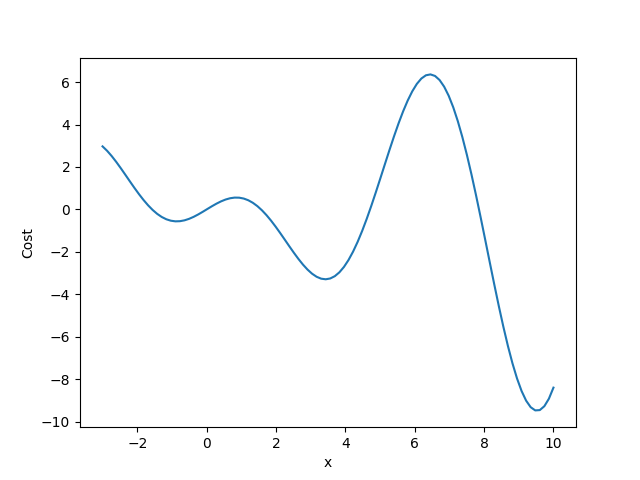
\includegraphics[width=0.8\textwidth]{figs/local_minima.png}
  \caption{Example showing multiple local minima using $y = x\cos x$, $x \in (-3,10)$}
  \label{fig:local_minima}
\end{figure}
\section{Neural Networks for learning inverses}
The iterative methods above invert the forward map each time for every measurement. An alternative would be to spend the computation time upfront and approximate a full inverse map once.

\subsection{Feed Forward Neural Network}
We use a fully-connected feed forward NN to approximate the inverse. Suppose we have a function $F: \mathbb{R}^N \rightarrow \mathbb{R}^M$ an approximate inverse is defined on the image of $F$, which we call $\hat{F}^{-1}$. We would like to find $y \in \mathbb{R}^N$ such that $y = \hat{F}^{-1}(x), x \in \mathbb{R}^M$. To do so, a feed-forward NN with $L$ hidden layers performs the composition shown in equation \eqref{eq:FFNN}, with $o_0 = x$ and $o_L = \hat{y}$:

\begin{align}
  \label{eq:FFNN}
  o_{i+1} &= \sigma \left(W_io_i + b_i\right) \text{,} i \in \{0,1,2,...l-2\} \\ 
  o_{L} &= W_{L-1}o_{l+1} + b_{l-1}
\end{align}
where $W_i$ and $b_i$ are the weight matrices and bias vectors (collectively the parameters $w$), and $\sigma$ is the nonlinear activation function.
We represent this approximation as $\hat{F}^{-1}_w: \mathbb{R}^M \rightarrow \mathbb{R}^N$, with $\hat{y} = \hat{F}^{-1}_w(x)$ 

The question then becomes how do we find the collection of parameters, $w$, which does this?

\subsection{Training a Neural Network}
Because we possess $F$ we can generate unlimited training data, a collection of labelled pairs, $(x_i,y_i)$. The goal of training is then to minimise the \emph{loss function} with respect to the parameters, $w$. The loss function is a performance metric for the network, and we will see in Section \ref{sec:res-network} that the choice of loss function is crucial to make a network perform well.
We minimise the loss using an optimiser, in our case the Adam optimiser \cite{kingma2017}. Generalisation is then assessed on a held-out test set never seen during training.


\newpage
\chapter{Methods}\label{chap:methods}
LM converges to a stationary point of the cost function, and which stationary point it reaches is determined by where it begins. So, how do we get into the right basin?

The solver is only as good as its initial guess. This chapter builds a NN based initialiser which then provides an initial guess for LM to allow it to converge to the correct stationary point. 

In this chapter, we follow a pipeline. First we figure out how to sample poses uniformly in $\Omega$. Then, these poses are fed into the forward model, yielding eight measuremnts. These 8 measurements are passed to a solver which gives back a predicted pose. The pipeline is shown in Figure \ref{fig:model_pipeline}. The first two stages of the pipeline exist only at training time. At inference time, the system only executes the three remaining stages.

Section \ref{sec:datagen} implements the forward map from Section \ref{sec:forward-map} in Python and shows how to sample poses uniformly. Section \ref{sec:error} defines the positional and angular errors used to evaluate the solvers. Section \ref{sec:methods-lm} describes the LM solver, and shows implementation considerations. Section \ref{sec:representation} examines how the pose should be represented as a target, particularly with respect to angle. Section \ref{sec:network} describes the architecture and training of the NN solver. Section \ref{sec:hybrid} joins the two halves. 


\begin{figure}
  \centering 
  \includegraphics[width=0.8\textwidth]{figs/model_pipeline.png}
  \caption{Pose estimation pipeline.}
  \label{fig:model_pipeline}
\end{figure}
\section{Data generation}\label{sec:datagen}

\subsection{Anser Simulation in Python}
We simulate the Anser system in Python, developing on a MATLAB simulation by Jaeger et al. \cite{jaeger2017}. \footnote{The implementation is available at
\url{https://github.com/pmccarthy3901/ansermodelling}. A mapping from the
sections of this chapter to the corresponding modules is given in
Appendix~\ref{app:code}.}
The forward model proceeds as follows:

\paragraph{Coil geometry}
First we generate the vertex coordinates for a square spiral PCB emitter coil. This is done in a local coordinate system and then copies are rotated and translated to place them in the global coordinate system. 

Each coil is a square which spirals in, it has $N$ turns per layer, the sidelength of the outermost square is $l$, the trace width is $w$, there is a line to line spacing of $s$ and the thickness of the PCB is $z_\mathrm{thick}$. After the coil has done $N_{\mathrm{turns}}$ turns on the upper layer, it is connected with a via to the lower layer where the coil spirals out again. 

\paragraph{Conversion from Local to Global Coordinates}
As all of the coils are the same shape, only one coil is generated, then it is copied a number of times into different places in space. 
The module selects an axis about which the rotation takes place. This is represented as an integer $(0,1,2) - (x,y,z)$. This works nicely because the rotation matrix can be generated using an even permutation of the axes. The module then applies the permuted rotation matrix to a copy of the input vector and then applies a translation.

\paragraph{Field Calculation}
The calculation of the magnetic field generated by the coils is done in \lstinline[style=python]|field_coil_calc|. It uses the linearity of the Biot-Savart line integral to calculate the total magnetic field due to the coils at an observer point as the sum of the contributions of each straight-line segment. It then implements equation \eqref{eq:biot_savart_final} to calculate the magnetic field.

%/\paragraph{Objective Function}

%The objective function \eqref{eq:objective_function} takes in the real observed measurement, and returns the difference between it and the measurement calculated using the simulation. It calculates the simulated measurement as:

%\begin{equation}
%  \mathbf{m}_\mathrm{sim} = \mathbf{H}_\mathrm{sim} \cdot \hat{n}_\mathrm{obs}
%\end{equation}
%where:
%\begin{itemize}
%  \item $\mathbf{H}_\mathrm{sim}$ is the simulated magnetic field 
%  \item $\hat{n}_\mathrm{obs}$ is the unit vector along the sensor axis.
%\end{itemize}
%Then, the objective function is calculated as: 
%\begin{equation}
%  \mathbf{r}:= \mathbf{m}_{\mathrm{sim}} - \mathbf{m}_{\mathrm{obs}}
%  \label{eq:objective_function}
%\end{equation}


\subsection{Sampling}
When generating data, it is important that our sampling space is uniform. For position, this is easy, we sample uniformly in the bounds of the box. The angle, however requires a bit more consideration.

\subsubsection{Sampling the position}
The Anser system operates in a 25x25x25cm box. 

Since the sensor coil is on a PCB that is $1.6$mm thick, the $z$ value has a minimum of $z = 0.0016$m. Therefore we sample uniformly within the bounds shown in Table \ref{tab:pos_bounds} 

\begin{table}
  \centering
  \begin{tabular}{lcc}
    \toprule
    Variable & Min (mm) & Max (mm) \\
    \midrule
    $x$ & $-125$ & $125$ \\
    $y$ & $-125$ & $125$ \\
    $z$ & $1.6$ & $250$ \\
    \bottomrule
  \end{tabular}
  \caption{Bounds of the sampling volume.}
  \label{tab:pos_bounds}
\end{table}
\subsubsection{Sampling the orientation}

Consider an area element $dA$ on the unit sphere, seen in Figure \ref{fig:unit_sphere}. Then the area element is $d A = \sin\theta d \theta d \phi$. Therefore, to uniformly sample on the sphere we must not sample uniformly in $\theta$, but rather in $\cos \theta$. The orientation sampling is shown in Table \ref{tab:angle_bounds}. As seen in Figure \ref{fig:orientation_sampling}, this leads to uniform sampling on the sphere. 

\begin{figure}
  \centering
  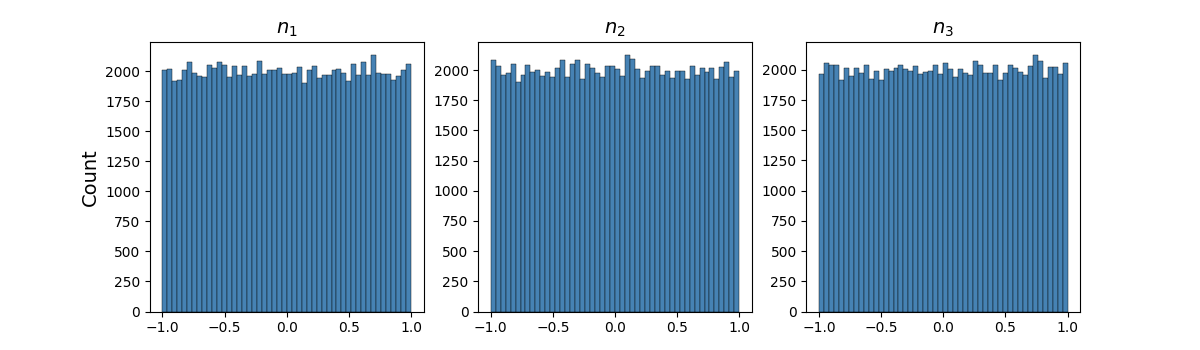
\includegraphics[width = 0.8 \textwidth]{figs/orientation_sampling.png}
  \caption{Orientation normal vectors sampled.}
  \label{fig:orientation_sampling}
\end{figure}

\begin{table}
  \centering
  \begin{tabular}{lcc}
    \toprule
    Variable & Min & Max \\
    \midrule
    $\cos\theta$ & $-1$ & $1$ \\
    $\phi$ & $0$ rad & $2\pi$ rad \\
    \bottomrule
  \end{tabular}
  \caption{Bounds of the orientation sampling volume.}
  \label{tab:angle_bounds}
\end{table}

\begin{figure}
  \centering
  \includegraphics[width = 0.4\textwidth]{figs/unit_sphere.png}
  \caption{Area element on the unit sphere. Reproduced from \cite{secil2023}}
  \label{fig:unit_sphere}
\end{figure}

\subsection{Dataset size, split, and normalisation}
The dataset consists of pose-measurement pairs. A subset of the poses are shown in space in Figure \ref{fig:sampled_poses}. The measurements are the model input and the pose is the regression target. The data is split 80/20 into training and validation sets, and the validation set is never seen during training. Models are then evaluated on a held out test set. The distribution of datapoints is shown in Table \ref{tab:data_splits}

\begin{table}
  \centering
  \begin{tabular}{ll}
    \toprule
    Split & Size \\
    \midrule
    $N_{\mathrm{train}}$ & $80,000$ \\
    $N_{\mathrm{val}}$ & $20,000$ \\
    $N_{\mathrm{test}}$ & $20,000$ \\
    \bottomrule
  \end{tabular}
  \caption{Data splits between training, validation, and testing data.}
  \label{tab:data_splits}
\end{table}
  

\begin{figure}
  \centering 
  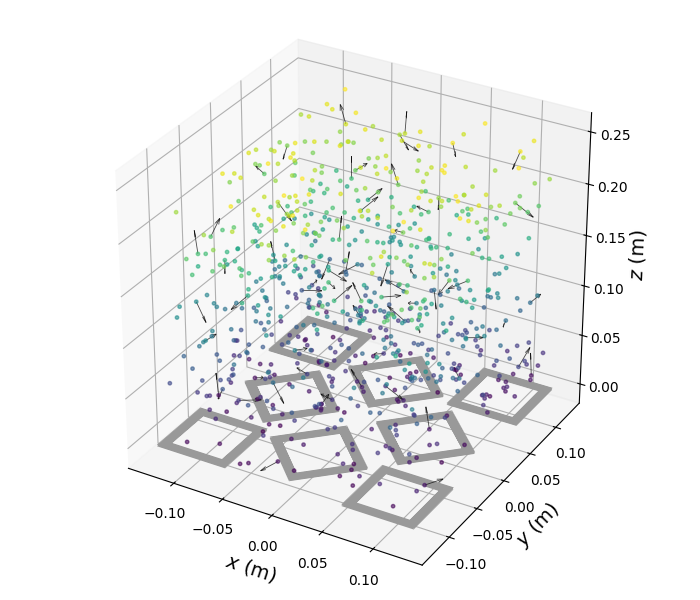
\includegraphics[width = 0.8 \textwidth]{figs/sampled_poses.png}
  \caption{800 poses sampled with some arrows indicating orientation.}
  \label{fig:sampled_poses}
\end{figure}

\section{Error metrics}\label{sec:error}
In order to quantify how "good" a particular model is, we need to define our errors. Since the pose has two components: position and orientation, we define an error on each. 

\subsection{Positional Error}
The positional error $e_p$ is defined using the euclidean distance between the true position, $x_\mathrm{true}$, and the predicted position, $x_\mathrm{pred}$.
\begin{equation}
  e_{p} := \left\Vert x_\mathrm{true} - x_\mathrm{pred} \right\Vert_2
\end{equation}

\subsection{Angular Error}
The angular error, $e_{\hat{n}}$, is defined in relation to the unit normal orientations, where $\hat{n}_\mathrm{true}$ is the true unit normal, and $\hat{n}_\mathrm{pred}$ is the predicted unit normal:
\begin{equation}
  e_{\hat{n}} := \arccos \left( \hat{n}_\mathrm{true} \cdot \hat{n}_\mathrm{pred} \right)
\end{equation}

\section{The Levenberg-Marquardt solver}\label{sec:methods-lm}
The previous chapter derived the LM update function \eqref{eq:lm}. This section describes the implementation and parameter choice. The chosen parameters were tuned against the validation set and are shown in Table \ref{tab:lm_parameters} 

\begin{table}
  \centering
  \begin{tabular}{ll}
    \toprule
    Property & Value \\
    \midrule
    $\lambda_0$ (Initial damping) & $10^{-5}$ \\
    $\lambda_{\max}$ (Maximum damping) & $10{^7}$ \\
    $\epsilon_{\mathrm{grad}}$ (Gradient threshold) & $10^{-5}$ \\
    Maximum Iterations & $100$ \\
    $h$ (Jacobian finite difference) & $10^{-5}$ \\
    \bottomrule
  \end{tabular}
  \caption{Parameters used in LM implementation.}
  \label{tab:lm_parameters}
\end{table}

\subsection{Implementation}
The solver is implemented in NumPy (\lstinline[style=python]|models/LM_solve.py|). Its components are as follows:

\paragraph{Jacobian.} As discussed in the previous chapter, we approximate the Jacobian using finite difference, as in \eqref{eq:jacobian}.

\paragraph{Scaling.} Following Marquardt's implementation \cite{marquardt1963}, the damping matrix is given by:
\begin{equation}
  D = \text{diag}(\max(\text{diag}(J^\top J), 10^{-12}))
\end{equation}
where the floor of $10^{-12}$ guards against a zero diagonal entry making $D$ singular and $\text{diag}$ is the function defined in Section \ref{sec:background-lm}

\paragraph{Constraint Handling.} At each iteration, constraints are applied to both the position and orientation. The position is clipped to within the box shown in Table \ref{tab:pos_bounds}. The orientations are handled by folding $\theta$ through the pole with a $\pi$ shift in $\phi$, and wrapping $\phi$. This keeps the orientation unchanged on the unit sphere and alters only its coordinates.

\paragraph{Damping.} Damping is done as in Section \ref{sec:background-lm}.

\paragraph{Stopping.} Iteration terminates when any of three conditions are met:
\begin{enumerate}
  \item the $l_{\infty}$ norm of the gradient falls below a threshold, $\epsilon_{\mathrm{grad}}$.
  \item The damping parameter, $\lambda$ exceeds $\lambda_{\mathrm{max}}$, indicating that no downhill step can be found. 
  \item A maximum number of iterations is reached, indicating that the solver cannot find a solution.
\end{enumerate}
Only the first of those three stopping criteria indicates success, and even then, the solver successfully reaching a minimum does not mean that it has successfully reached the correct minimum. Therefore we have to define convergence.

We say that a solution has converged if for some $\epsilon_p$ and some $\epsilon_n$ "acceptable errors":
\begin{align*}
  e_p &< \epsilon_p \\
  e_{\hat{n}} &< \epsilon_n 
\end{align*}

\section{Representing the pose}\label{sec:representation}
The pose contains two angles, and how they are represented as regression targets matters more than it first appears. Regressing against $\theta$ and $\phi$ directly has three problems. First, $\phi$ is periodic: $\phi = 0.01$ and $\phi = 2\pi - 0.01$ are only separated by $0.02$ rad, however a naive loss would heavily punish such a situation. The second problem is with $\phi$: at the poles $\theta \in \{0,\pi\}$, $\phi$ is not defined. The third problem is more general: squared error in the angles is not a distance on the sphere. The metric induced on the unit sphere, $S^2$, by the parametrisation carries an extra factor of $\sin^2\theta$:
\begin{equation}
  ds^2 = d\theta^2 + \sin^2\theta \, d\phi^2 
\end{equation}

For these reasons, it becomes natural to represent the orientation not in terms of angles, but in terms of the unit normal itself:

\begin{equation}
  \hat{n}(\theta,\phi) = \begin{bmatrix} \sin\theta\cos\phi \\ \sin\theta\sin\phi \\ \cos\theta \end{bmatrix}
\end{equation}
The normal vector is smooth, unique, and has no wrap-around. We therefore train networks whose target is the vector:
\begin{equation}
  t = (x,y,z,n_1,n_2,n_3)
\end{equation}
where $n_i$ is the unit normal in the $i$th direction.

This argument, however, does not apply to the LM solver of Section \ref{sec:methods-lm}, which continues to operate in the $(\theta,\phi)$ regime. This is because an iterative solver initialised near its solution does not encounter these problems and, conversely, if we were to regress against the unit normal we would have the issue of having 6 parameters for 5 degrees of freedom meaning that $J^{\top} J$ would not be invertible, contradicting the exact condition that LM needs.  


\section{Neural Network Solver}\label{sec:network}
Section \ref{sec:methods-lm} establishes that the LM solver needs a good initial guess to converge. This section builds a NN solver, the main advantage of which is its ability to learn the global configuration of the system and thus work on a "cold start". This section shows the choice of architecture, loss function, and training methods.
\subsection{Neural Network Architecture}
The NN solver uses a basic feed-forward-neural-network which takes the 8 input measurements and outputs the 6 dimensional pose $(x,y,z,n_1,n_2,n_3)$. The NN architecture is shown in Table \ref{tab:architecture} 

\begin{table}
  \centering
  \begin{tabular}{ll}
    \toprule
    Property & Value \\
    \midrule
    Input dimension       & 8 (measurements) \\
    Output dimension      & 6 ($x, y, z, n_1, n_2, n_3$) \\
    Hidden layers         & 3 \\
    Units per layer       & (256,256,256) \\
    Activation            & tanh \\
    \bottomrule
  \end{tabular}
  \caption{Network architecture.}
  \label{tab:architecture}
\end{table}
\subsection{Choice of loss function}\label{sec:methods-loss}
In Section \ref{sec:error} we defined two errors: $e_p$, the positional error, and $e_{\hat{n}}$, the angular error. Now we must define a loss function. The only problem is that these errors operate on completely different scales. Given the bounds of our box, $e_p$ varies between $0$ and $w_p$, where $w_p$ is the diagonal length of the box, and $e_{\hat{n}}$ varies between $0$ and $w_{\hat{n}} = \pi$. To give equal weight to both components we define our loss, $\mathcal{L}$, as the weighted sum between squares of the two as follows: 
\begin{equation}
  \mathcal{L} = e_p^2 + \frac{w_p^2}{w_{\hat{n}}^2} e_{\hat{n}}^2
  \label{eq:loss}
\end{equation}
This weight is chosen such that the two terms have equal range over the sampling volume.
\subsection{Neural Network Training}
The network is trained with the Adam optimiser \cite{kingma2017} to minimise \eqref{eq:loss} over the dataset described in Section \ref{sec:datagen}, using the settings and hyperparameters described in Table \ref{tab:training}

The learning rate uses a cosine scheduler \cite{loshchilov2017}, decaying from its initial value to zero, as in equation \eqref{eq:cosine_annealing} with parameters in Table \ref{tab:training}, where $t$ is the current epoch and $\eta_0$ is the learning rate at the 0th epoch. This allows for a high learning rate at the start, which then decays smoothly at every epoch. This means that at the start the model learns quickly, and at the end the model has sufficiently small learning rate to not oscillate around the minimum. 

\begin{equation}
  \eta_{t+1} = \eta_{\mathrm{min}} + (\eta_t - \eta_{\mathrm{min}}) \frac{1 + \cos \left( \frac{t+1}{T_{\mathrm{max}}}\pi \right)}{1 + \cos \left( \frac{t}{T_\mathrm{max}} \pi \right)}
 \label{eq:cosine_annealing} 
\end{equation}
\begin{table}
  \centering
  \begin{tabular}{ll}
    \toprule
    Parameter & Value \\
    \midrule
    Optimiser       & Adam \\
    Schedule        & Cosine Annealing \\
    Batch size      & 32 \\
    Epochs          & 200 \\
    $\eta_{0}$ & $10^{-3}$ \\
    $\eta_{\mathrm{min}}$ & $0$ \\
    $T_{\max}$ & $200$ \\
    \bottomrule
  \end{tabular}
  \caption{Training configuration.}
  \label{tab:training}
\end{table}
\section{Hybrid Model}\label{sec:hybrid}
Sections \ref{sec:methods-lm} and \ref{sec:network} present a LM based solver and a NN solver, respectively. The shortcomings of these two solvers are complementary. A hybrid model combines these two, feeding the output of the NN model into a LM solver. This allows the NN to provide a good initialisation for the LM solver to further refine.

\subsection{Coupling the two solvers}
The two components operate in different parametrisations. The NN uses $(x,y,z,n_1,n_2,n_3)$ and the LM solver uses $(x,y,z,\theta,\phi)$. This means that before feeding the NN output into the LM solver, we have to convert the parametrisation.

Given the predicted normal $\hat{n} = (n_1,n_2,n_3)$, normalised to unit length, the corresponding $\theta$ and $\phi$ are given by: 
\begin{align*}
  \theta &= \arccos(n_3) \\
  \phi &= \operatorname{atan2}(n_2,n_1)
\end{align*}
where $\operatorname{atan2}$ is the two argument arctangent defined by:
\begin{equation}
  \operatorname{atan2}(y,x) =
  \begin{cases}
    \arctan\!\left(\frac{y}{x}\right)         & \text{if } x > 0, \\
    \arctan\!\left(\frac{y}{x}\right) + \pi   & \text{if } x < 0 \text{ and } y \geq 0, \\[6pt]
    \arctan\!\left(\frac{y}{x}\right) - \pi   & \text{if } x < 0 \text{ and } y < 0, \\[6pt]
    +\frac{\pi}{2}                            & \text{if } x = 0 \text{ and } y > 0, \\[6pt]
    -\frac{\pi}{2}                            & \text{if } x = 0 \text{ and } y < 0, \\[6pt]
    \text{undefined}                          & \text{if } x = 0 \text{ and } y = 0.
  \end{cases}
  \label{eq:atan2}
\end{equation}
The use of $\operatorname{atan2}$ instead of the normal arctangent allows us to both get in the correct quadrant and also mitigates against the singularity caused when $n_1 = 0$.

Now we can build our hybrid pipeline. The pipeline is shown in Figure \ref{fig:hybrid_pipeline}

\begin{figure}
  \centering 
  \includegraphics[width = 0.8 \textwidth]{figs/hybrid_pipeline.png}
  \caption{Data pipeline for hybrid model}
  \label{fig:hybrid_pipeline}
\end{figure}


\newpage
\chapter{Results}\label{chap:results}

Chapter \ref{chap:methods} built three solvers. The LM solver, the NN solver, and the hybrid solver. This chapter evaluates each of the three solvers on a held-out test set and compares them against one another. 

The chapter contains three steps. Section \ref{sec:results-lm} measures how good an initialisation must be for LM to converge, Section \ref{sec:res-network} measures how good the network's predictions are, and Section \ref{sec:three_way} tests whether the network initialisation is good enough for the LM solver to converge. We close the chapter by discussing the implications of these results.

\section{Experimental Setup}
All models are evaluated on the same held out test set consisting of $N_{\mathrm{test}}$ datapoints, generated separately from the training/validation datapoints. The data splits are shown in Table \ref{tab:data_splits}.  


\subsection{Hardware Setup}
Training and inference times are reported throughout this chapter. All computation is done on the same machine with specifications shown in Table \ref{tab:comp_specs}. Models are trained purely on the CPU. In reporting we use the CPU time, not the wall time, because some processes are singlethreaded whereas others are multithreaded. For example, NN training is multi-threaded, whereas LM inference is single-threaded. 

\begin{table}
  \centering
  \begin{tabular}{ll}
    \toprule
    Component & Model \\
    \midrule
    CPU  & AMD Ryzen 5 1600x \\
    RAM  & 32GB DDR4 2133MT/S \\
    \bottomrule
  \end{tabular}
  \caption{Computer specifications for training and inference}
  \label{tab:comp_specs}
\end{table}

\subsection{Convergence Criteria}\label{sec:conv_criteria}
In Section \ref{sec:methods-lm} we define two constants, $\epsilon_p$ and $\epsilon_n$, which dictate when we consider a run to have \emph{converged}. In this chapter, we use the values shown in Table \ref{tab:conv_criteria}. A solve is said to have converged if the positional and angular errors are both less than $\epsilon_p$ and $\epsilon_n$, respectively.

\begin{table}
  \centering
  \begin{tabular}{ll}
    \toprule
    Parameter & Value \\
    \midrule
    $\epsilon_p$  & 1\,mm \\
    $\epsilon_n$ & 1$^\circ$ \\
    \bottomrule
  \end{tabular}
  \caption{Convergence criteria for results reporting.}
  \label{tab:conv_criteria}
\end{table}

\section{The Levenberg-Marquardt Solver}\label{sec:results-lm}
Section \ref{sec:methods-lm} shows how we implement the LM solver. This section shows its performance and motivates the need for NN initialisation.

\subsection{Basin Sweep}
We want to know how accurate an initialisation must be before LM can recover the pose. We therefore work out how "bad" an initialisation can be to give a desired convergence rate. 
\paragraph{Method -} $N_{\mathrm{bs}} = 200$ poses are sampled from the held-out test set with a fixed seed. We then perform two independent perturbation sweeps: A positional sweep and an angular sweep. The position perturbation is generated by picking a random direction via Gaussian sampling. Then normalising that vector and multiplying by the perturbation distance, $d$. The angular perturbation requires some consideration. 

If we want to perturb an orientation vector $\hat{n} = (n_1,n_2,n_3)$ by an angle $\alpha$, we generate a random vector from a Gaussian distribution $v \sim \mathcal{N}(0,I_3)$. Then we project $v$ onto the plane perpendicular to $\hat{n}$, as in equation \eqref{eq:proj_v_n}. After this, we normalise $v_{\perp}$ and rotate by $\alpha$ in the direction of $v_{\perp}$ as in equation \eqref{eq:rotation}.

\begin{equation}
  v_{\perp} = v - (v \cdot \hat{n}) \hat{n}
  \label{eq:proj_v_n}
\end{equation}

\begin{equation}
  \hat{n}_\mathrm{pert} = \cos(\alpha) \hat{n} + \sin(\alpha) (v_{\perp} / \left\vert v_{\perp} \right \vert)
  \label{eq:rotation}
\end{equation}


For each of the sweeps, the convergence rate is calculated as in Section \ref{sec:conv_criteria}.

\paragraph{Positional Sweep -} The position is swept from $d = 0$ to $d = 150$mm. Figure \ref{fig:pos_sweep} shows that as the perturbation magnitude increases, there is a steady decrease in the convergence rate, with no sharp dropoff. This suggests that there are no sharp boundaries contrary to what one might expect of a Newton-type method. 
\begin{figure}
  \centering 
  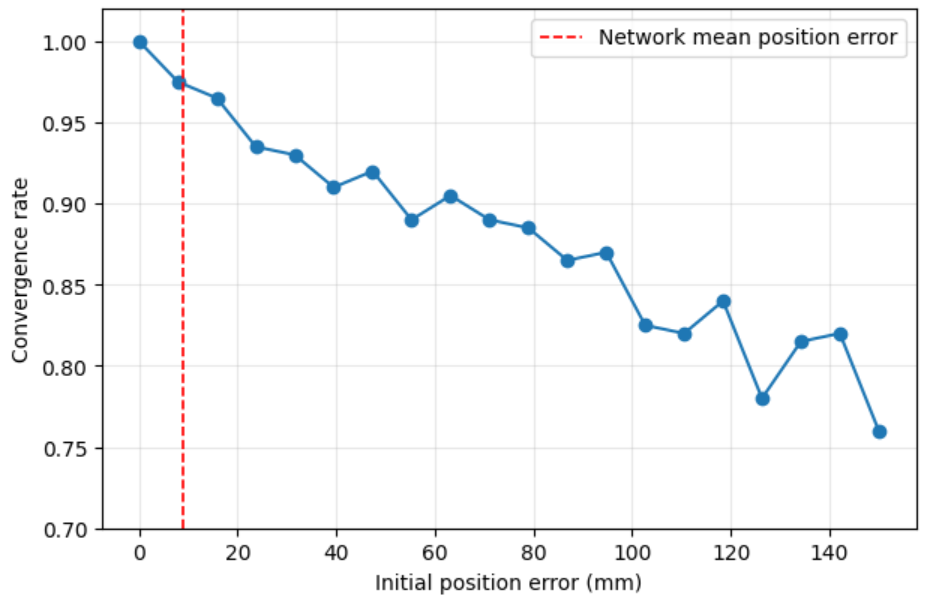
\includegraphics[width = 0.8 \textwidth]{figs/pos_sweep.png}
  \caption{Convergence rate against positional perturbation. The dashed line marks the mean positional error of the trained NN seen in Section \ref{sec:res-network}.}
  \label{fig:pos_sweep}
\end{figure}

\paragraph{Angular Sweep -} The angle is swept from $\alpha = 0$ to $\alpha = 90^{\circ}$. Figure \ref{fig:angle_sweep} shows the same story as the positional sweep, steady decrease with no sharp dropoff. We do note that the angle is a lot more forgiving than position, retaining a 97.5\% convergence rate up to $\alpha = 42.6^\circ$. This is because the equation \eqref{eq:forward} depends on $1/r^{3}$ whereas the orientation angle only enters through the dot product.

\begin{figure}
  \centering
  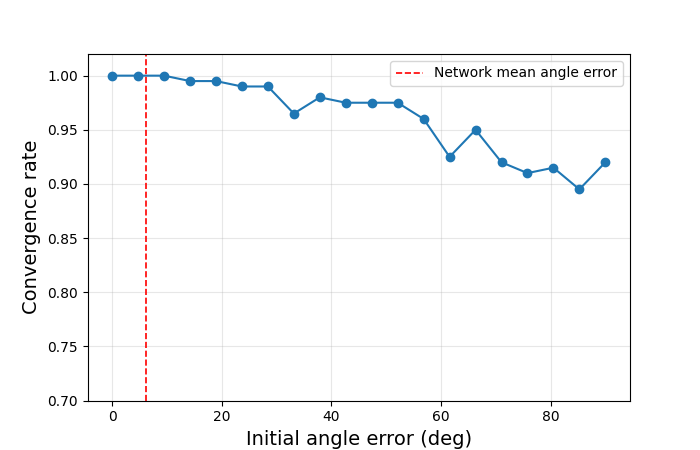
\includegraphics[width = 0.8\textwidth]{figs/angle_sweep.png}
  \caption{Convergence rate against angular perturbation. The dashed line marks the mean angular error of the trained NN.}
  \label{fig:angle_sweep}
\end{figure}

What is interesting in both the positional and angular sweeps is that the failure is discrete. Either the solver converges to machine precision $\sim 10^{-14} \mathrm{mm/}^\circ$ or else it is off by a large number. This is seen when comparing the mean, median, and 95\% error. For example, in the positional perturbation with $d = 86.8$ mm we get a mean positional error of 8.13mm but a median positional error of $1.8*10^{-11}$mm, suggesting that a few outliers inflate the mean. This is further confirmed by the 95\% error of 56.3mm, showing that either the solver works or it does not, there is no slow dropoff in error. This is also shown in Figure \ref{fig:pos_sweep_errors}.


\begin{figure}
  \centering 
  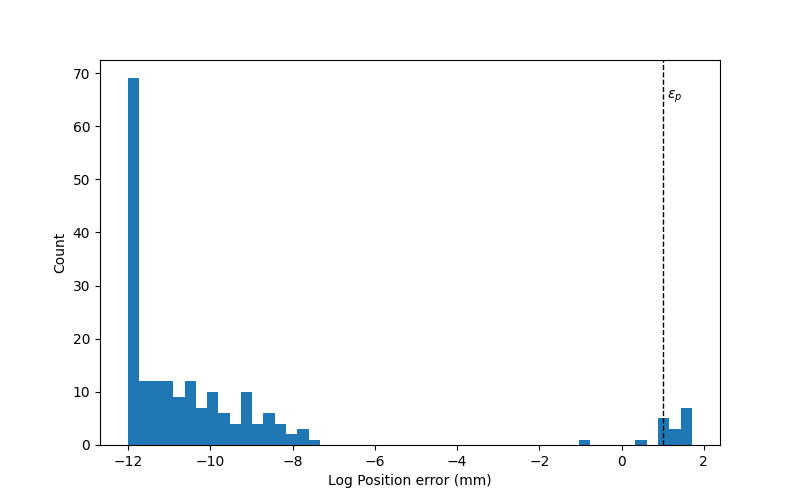
\includegraphics[width = 0.8\textwidth]{figs/pos_sweep_errors.png}
  \caption{Histogram of log positional error for $d = 47.4$mm showing two error classes, failure and convergence.}
  \label{fig:pos_sweep_errors}
\end{figure}

\section{Network Training}\label{sec:res-network}
\subsection{Training Configuration}
In training the network, a number of tuning choices were made against the validation set. First, and most importantly, the network uses the 6-dimensional $(x,y,z,n_1,n_2,n_3)$ pose representation rather than the 5-dimensional $(x,y,z,\theta,\phi)$ representation. Secondly the "PoseLoss" loss function described in Section \ref{sec:methods-loss} was used, instead of MSE. Third, the learning rate was varied using a cosine annealing scheduler, as described in section \ref{sec:network}. Each of these training configurations are shown in  Table \ref{tab:training_config} 
\begin{table}
  \centering
  \begin{tabular}{llllll}
    \toprule
    Name & Target & Loss & LR Scheduler & Optimiser & Epochs\\
    \midrule
    Base & $(\theta,\phi)$ & MSE & None & Adam & 200  \\
    Normal & $\hat{n}$ & MSE & None & Adam & 200\\
    PoseLoss & $\hat{n}$ & PoseLoss & None & Adam & 200 \\
    Final & $\hat{n}$ & PoseLoss & Cosine & Adam & 200 \\
    \bottomrule
  \end{tabular}
  \caption{Experimental Design of NN models.}
  \label{tab:training_config}
\end{table}
\begin{table}
  \centering
  \begin{tabular}{lll}
    \toprule
    Name & Mean Pos Error (mm) & Mean Angular Error (deg)  \\
    \midrule
    Random Pair & 165 & 90 \\
    Centre Predictor & 120 & 90 \\
    Base & 135 & 87.1  \\
    Normal & 139 & 47.7 \\
    PoseLoss & 21.3 & 8.67 \\
    Final & 9.2 & 6.43 \\
    \bottomrule
  \end{tabular}
  \caption{Test set performance of NN models.}
  \label{tab:nn_results}
\end{table}

\paragraph{Base -}Table \ref{tab:nn_results} shows that the base model performs only marginally better than a baseline estimator i.e. it is not much better than a random guess. The expected positional and angular error for two randomly sampled points were estimated using a Monte Carlo simulation drawing from the test set. More interestingly, the base model actually performs worse on position than just guessing the centre of the box every time. This tells us that the base model learns nothing about the orientation and almost nothing about the position.


\paragraph{Normal -}The "Normal" configuration improves the angular error to about half of baseline but left the positional error the same, suggesting that the change to normal parametrisation allows the network to start learning the orientation configuration of the system.

\paragraph{PoseLoss -}The biggest change happens when we change the loss function from MSE to our PoseLoss, reducing positional error by a factor of $6.5$ and angular error by a factor of $5.5$. This change allows the network to actually learn against angular error and also weights the positional and angular error more equally.

\paragraph{Final -}Further refinement is achieved through the use of Cosine learning rate scheduling, allowing training to slow down towards the end, learning the finer details of the data. 
\subsection{Final Model}
The Final NN model, with configuration seen in Table \ref{tab:training_config} was chosen to be used. The number of epochs was chosen to be 200 because by 200 the error on the validation set started plateauing. This plateau can be seen in Figure \ref{fig:training_curves}. 

\begin{figure}
  \centering 
  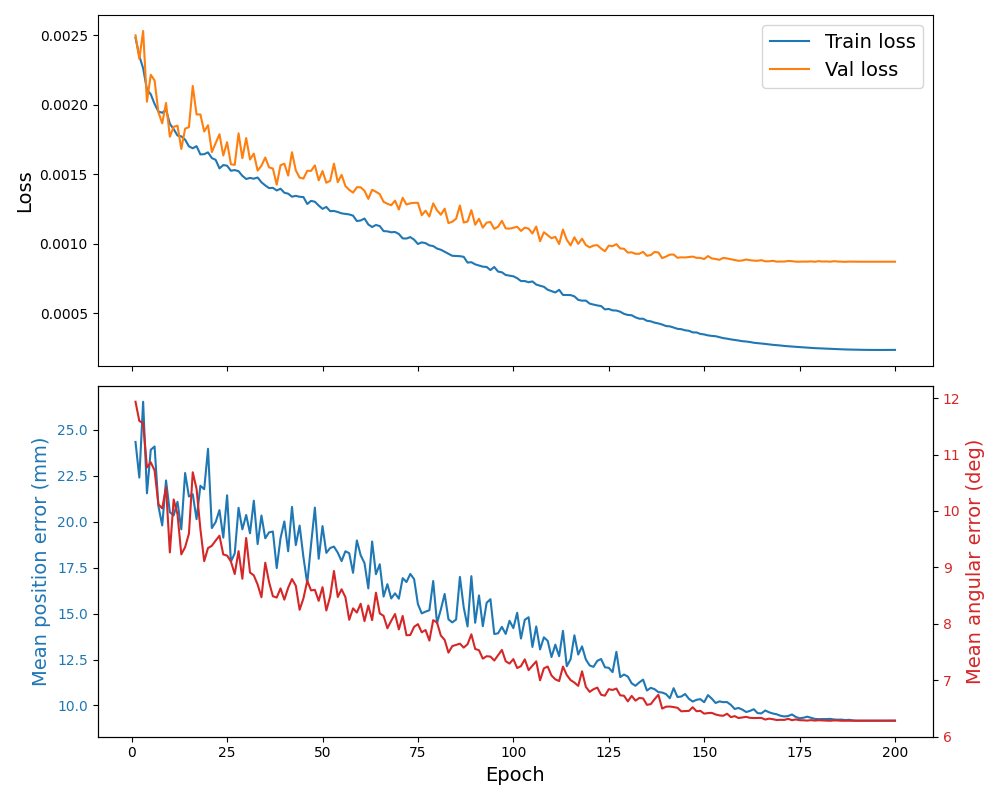
\includegraphics[width = 0.8\textwidth]{figs/training_curves.png}
  \caption{Loss curves and error curves on the validation set}
  \label{fig:training_curves}
 \end{figure}

 \section{Three-way Comparison}\label{sec:three_way}

All three solvers are evaluated on the same held-out test set of 20,000 datapoints. The LM solver uses the same parameters as in section \ref{sec:methods-lm}. The LM model is initialised from the centre of the box with the orientation in the $\hat{z}$ direction. The hybrid solver uses the same solver parameters and differs only in where it starts. The hybrid solver uses the output of the NN as a start point. The results of this test are shown in Table \ref{tab:three_way}. 


\begin{table}
  \centering
  \begin{tabular}{lrrr}
    \toprule
    & LM (cold start) & Network & Hybrid \\
    \midrule
    Mean position error (mm)        & 9.71 & 9.20 & 1.12 \\
    Median position error (mm)      & $1.5\times10^{-11}$ & 7.33 & $3.8\times10^{-12}$ \\
    95th pct.\ position error (mm)  & 64.2 & 21.7 & 1.67 \\
    \addlinespace
    Mean angular error ($^\circ$)       & 8.95 & 6.43 & 1.89 \\
    Median angular error ($^\circ$)     & $5.3\times10^{-12}$ & 3.62 & $1.2\times10^{-12}$ \\
    95th pct.\ angular error ($^\circ$) & 79.5 & 20.9 & 2.46 \\
    \addlinespace
    Convergence rate & 0.859 & 0.0008 & 0.947 \\
    Training time    & --- & 2h 32m 49s & --- \\
    Inference time   & 16m 3s & 361\,ms & 5m 45s \\
    \bottomrule
  \end{tabular}
  \caption{Performance of the three solvers on the held-out test set of
  20{,}000 poses.}
  \label{tab:three_way}
\end{table}

The LM and NN solvers obtain similar mean positional errors, however these solvers operate very differently. The LM solver is extremely bimodal, it either converges to a tiny error on the order of $10^{-11}$mm or else it completely fails. This behaviour is seen when we look at the median and 95th percentile position errors. The NN, on the other hand, has a unimodal distribution of positional errors, with mean, median, and 95th percentile error on similar scales. This suggests that NN performs similarly on almost all poses. This behaviour is seen in Figures \ref{fig:three_way_pos} and \ref{fig:three_way_angle}.

\begin{figure}
  \centering 
  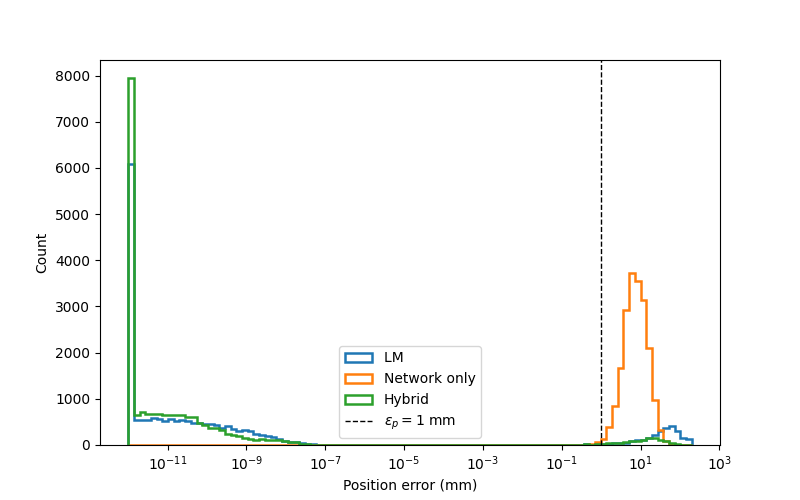
\includegraphics[width=0.8\textwidth]{figs/three_way_pos.png}
  \caption{Histogram of positional errors for each of the three solvers.}
  \label{fig:three_way_pos}
\end{figure}

\begin{figure}
  \centering 
  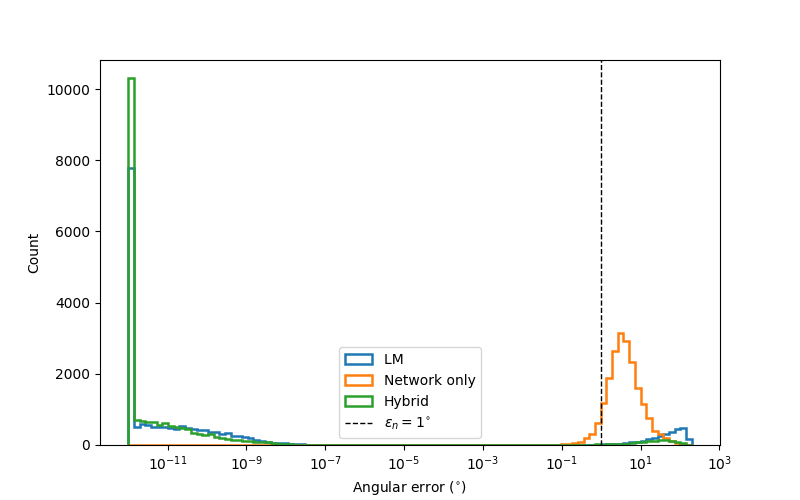
\includegraphics[width = 0.8\textwidth]{figs/three_way_angle.png}
  \caption{Histogram of angular errors for each of the three solvers.}
  \label{fig:three_way_angle}
\end{figure}

The goal of the Hybrid solver is to push the LM into the low error mode. We see in Table \ref{tab:three_way} that it succeeds in this goal. It decreases the rate of non-convergence by a factor of $2.66$. The median errors of the Hybrid solver remain similar to that of the LM solver, however the mean and 95th percentile errors decrease drastically. Looking at the rightmost peaks in Figures \ref{fig:three_way_pos} and \ref{fig:three_way_angle} shows us that the Hybrid has fewer failures and even when it fails the error is smaller than the LM solver. The Network initialisation does not make LM more accurate, it just makes LM succeed more often.

The LM solver does not require any training, all of the compute is done at inference time. The NN solver on the other hand, does a vast majority of the compute at training time, and only a small amount at inference time. Table \ref{tab:three_way} shows that the LM solver requires two orders of magnitude more inference time than the NN, the NN's cost is instead paid at training time, taking over two hours to train. The Hybrid solver inherits the compute done in NN training, making inference faster by making it do fewer iterations. On the test-set it takes the Hybrid solver just over five minutes to solve all $N_{\mathrm{test}}$ poses. This is almost three times faster than the LM solver. This means that after approximately 300,000 poses the Hybrid solver will reach its break-even point. Further advocating for the Hybrid, inference time should be valued higher than training time, as training only has to be done once and can be done on a powerful computer rather than on the system itself. 


\section{Discussion of Results}
\subsection{Does the basin sweep explain the Hybrid?} The basin sweep predicts convergence rates $r_p$ and $r_\theta$ for the network's positional and angular error, respectively. Under independence, the Hybrid's convergence rate would be the product $r_p r_\theta$. However, the observed hybrid rate $r_h$ falls short of this prediction. Two possible reasons present themselves. Firstly, the basin sweep is only calculated on far fewer points than the Hybrid analysis, so the difference in convergence rates might be an artifact of the different sample sizes. The second possible reason is that the composition of errors might not be independent. 

We test the first explanation by constructing a hypothesis test. We test the null hypothesis that both are estimates of the same underlying rate. The resulting z-score \eqref{eq:z-score} with values from Table \ref{tab:z-scoring} give a $p < 0.05$. We therefore reject the null hypothesis at 5\% significance. This suggests that the composition of errors is therefore not independent. This means that the sweeps explain why the Hybrid performs well, but cannot predict how well the Hybrid performs. 

\begin{table}
  \centering 
  \begin{tabular}{lll}
    \toprule 
    Quantity & Symbol & Value \\
    \midrule 
    Positional error convergence rate & $r_p$ & 0.975 \\
    Angular error convergence rate & $r_\theta$ & 1.00 \\
    Observed Hybrid rate & $r_h$ & 0.947 \\
    \bottomrule 
  \end{tabular}
  \caption{Basin sweep vs. observed Hybrid convergence rates.}
  \label{tab:z-scoring}
\end{table}
\begin{equation}
  z = \frac{r_pr_\theta - r_h}{\sqrt{\frac{r_pr_\theta \times (1-r_pr_\theta)}{N_{\mathrm{BS}}}+\frac{r_h \times (1-r_h)}{N_\mathrm{test}}}} = 2.51 
  \label{eq:z-score}
\end{equation}


\subsection{Consistency between basin sweep and LM solver} The LM solver initialises at the box centre, with mean distance to a test pose of $\bar{d}_{\mathrm{LM}}$ and gives a convergence rate of $r_\mathrm{LM}$. The basin sweep gives a convergence rate of $r_{\mathrm{BS}}$ when the pose is perturbed by a similar distance $d_\mathrm{BS}$. Using the same test as in the previous section with values from Table \ref{tab:conv_rates_cold}, we get a $p$ value of $0.64$. The two are statistically indistinguishable from one another at this sample size, suggesting that the two experiments are consistent with one another.
\begin{table}
  \centering 
  \begin{tabular}{lll}
    \toprule 
    Quantity & Symbol & Value \\
    \midrule 
    LM mean distance to test pose & $\bar{d}_\mathrm{LM}$ & $\approx 120$mm \\
    Closest basin sweep perturbation to LM mean & $d_\mathrm{BS}$ & $118$mm \\
    LM Cold start convergence rate & $r_\mathrm{LM}$ & $0.859$ \\
    Equivalent basin sweep convergence rate & $r_\mathrm{BS}$ & $0.84$ \\
    \bottomrule 
  \end{tabular}
  \caption{Basin sweep vs. cold start LM convergence rates.}
  \label{tab:conv_rates_cold}
\end{table}



\subsection{Precision vs Reliability} Throughout this chapter, two key attributes distinguish the solvers: precision and reliability. LM is very precise, when it receives a good initialisation. It is not very reliable though. If it does not receive a good initialisation it completely fails. For example, in the basin sweep with a large value of $d$, the 95th percentile positional error is exactly $d$, meaning that the solver did nothing to the initial guess. The NN on the other hand is not very precise, with positional errors consistently on the order of $9$mm. However, it is extremely reliable, achieving a positional error less than $21.7$mm 95\% of the time. The function of the Hybrid solver is that it inherits precision from the LM solver, and reliability from the NN solver. None of the improvements in this chapter came from giving the model more training data or increasing the model's capacity. One came from the choice of loss function, and one came from choosing to use the NN to initialise LM.


\newpage 
\chapter{Conclusion}\label{chap:conclusion}

\section{Summary of Findings}

This thesis asked how an LM pose solver can be reliably initialised when no previous pose exists. To answer this question, we reimplemented the Anser forward model in Python, characterised the solver's convergence as a function of initialisation quality, trained an NN to predict pose directly, and combined the two into a hybrid solver. 

The basin sweeps showed that convergence degrades as the initialisation error increases, and that failure is discrete. The LM solver either converges or fails outright. The network alone is reliable but imprecise. Its errors are unimodal and never reach the desired convergence tolerances. The two solvers are therefore complementary. The hybrid solver derived by combining the two retains the precision of the LM solver, but allows the NN initialisation to provide increased reliability. 

\section{Limitations and Future Work}

The most significant limitation is that all results are purely simulated. This thesis validates the solver against the forward model, not the model against reality. Next steps should include validating the Hybrid solver against physical data. As the results are simulated, they contain no noise. Real EMT systems experience two types of noise. Random noise, and systematic noise. Random noise, arising from the sensitivity of the sensors and compounding errors in the data pipeline, and systematic noise which comes from nearby conductive or ferromagnetic objects. These two forms of noise together are the dominant error source in real EMT deployments \cite{sorriento2020}. 

A single, basic NN architecture was used. There was no capacity study. Future work could include testing more complex models, seeing how much training data is needed, and varying model capacity to tune for accuracy and computation time in inference.

This thesis uses a finite-difference Jacobian. However, if the forward map were reimplemented in PyTorch, we could have used autograd to obtain an analytic Jacobian. This would remove the step-size parameter $h$, and its associated truncation error


\newpage 
\chapter{Code}\label{app:code}
The implementation is available at \url{https://github.com/pmccarthy3901/posesolving}. 
Table \ref{tab:code_map} maps the sections of the thesis to the corresponding Python modules.


\begin{table}
  \centering 
  \begin{tabular}{lll}
    \toprule 
    Section & Module & Contents \\
    \midrule 
    \ref{sec:anser_sim} & \lstinline[style=python] |anser/| directory & Anser forward model simulation. \\
    \ref{sec:dataset} & \lstinline[style=python] |data/build_dataset.py| & Dataset generation. \\
    \ref{sec:error} & \lstinline[style=python] |models/train.py| & Error metrics. \\
    \ref{sec:methods-lm} & \lstinline[style=python] |models/LM_solve.py| & LM implementation. \\
    \ref{sec:network} & \lstinline[style=python]|models/FFNN_network.py| & NN configuration. \\
    \ref{sec:methods-loss} & \lstinline[style=python] |models/train.py| & Loss function. \\
    \ref{sec:nn_training} & \lstinline[style=python] |models/train.py| & Network training. \\
    \ref{sec:hybrid} & \lstinline[style=python] |data/reparametrisation.py| & Reparametrisation. \\
    \ref{sec:results-lm} & \lstinline[style=python] |demos/basin_sweep.ipynb| & Basin sweep. \\
    \ref{sec:three_way} & \lstinline[style=python] |demos/solver_demos.ipynb| & Three-way comparison. \\
    \bottomrule 
  \end{tabular}
  \caption{Mapping between thesis sections and Python modules.}
  \label{tab:code_map}
\end{table}



\newpage
\bibliographystyle{unsrt}
\bibliography{references}


\end{document}
